% STANDARD PACKAGES
\documentclass[12pt, twoside]{article}

\usepackage{styles}

\begin{document}

\begin{titlepage}
    \centering
    \vspace*{\fill}
    \vspace*{-5cm} % Move up by 2cm
    {\LARGE CMPUT 653: Foundations of Reasoning \newline in LLMs Lecture Notes\par}
    \vspace{0.6cm}
    {\Large Siddhartha Chitrakar\par}
    \vspace{0.5cm}
    {\large \today\par}
    \vspace*{\fill}
\end{titlepage}

% Roman Page Numbering for Preface
\pagenumbering{roman}
\setcounter{page}{2}

\newpage

% ↓↓↓ REMOVE SECTION FROM HEADER ↓↓↓
\fancypagestyle{RemoveHeader}{
  \fancyhf{} % clear all headers/footers
  \fancyhead[R]{\thepage} % keep page number on top right
}
\thispagestyle{RemoveHeader}
% ↑↑↑ REMOVE SECTION FROM HEADER ↑↑↑

\tableofcontents
\newpage

% ↓↓↓ SHOW CORRECT SECTION FROM HEADER WITHOUT # ↓↓↓
\markboth{Preface}{Preface}
\section*{Preface}
\addcontentsline{toc}{section}{Preface}

\subsection*{Symbols and Remark on Notation}
\addcontentsline{toc}{subsection}{Symbols and Remark on Notation}
% ↑↑↑ SHOW CORRECT SECTION FROM HEADER WITHOUT # ↑↑↑


Insert Preface.

\subsection*{Acknowledgments}
\addcontentsline{toc}{subsection}{Acknowledgments}

Insert Acknowledgments.

\newpage

% Normal Page Numbering for Main Text
\pagenumbering{arabic}
\setcounter{page}{1}
\makelecturetitle{\href{https://youtu.be/3bG2Dy7Du0Y?si=GEyV1hcv_MvwvY_Z}{Lecture 1 Video}, \href{https://youtu.be/DR8bQPoRlX8?si=h5u-xZKmQuMA6K5N}{Lecture 2 Video}}{Csaba Szepesvári}{Siddhartha Chitrakar}{Sep. 3 and Sep. 5 2025}

% ↓↓↓ REMOVE SECTION FROM HEADER ↓↓↓
\fancypagestyle{RemoveHeader}{
  \fancyhf{} % clear all headers/footers
    \fancyhead[R]{\thepage} % keep page number on top right
}
\thispagestyle{RemoveHeader}
% ↑↑↑ REMOVE SECTION FROM HEADER ↑↑↑

% ↓↓↓ SHOW CORRECT SECTION FROM HEADER WITHOUT # ↓↓↓
\markboth{Lecture 1 and 2: Modelling Sequences}{Lecture 1 and 2: Modelling Sequences}
\stepcounter{section}
\section*{Lecture 1 and 2: Modelling Sequences}
\addcontentsline{toc}{section}{1. Modelling Sequences}
% ↑↑↑ SHOW CORRECT SECTION FROM HEADER WITHOUT # ↑↑↑

\textit{Note:} Lecture 1 contains errors due to reusing the notation $p$ for different meanings. Lecture 2 corrected this; [*timestamp] used to link second lecture.


We use \textbf{probabilistic sequence models} to model sequences. Exercise \ref{ex:1.1}, \ref{ex:1.2} intuitively explain why we use this, but first we introduce some notation:

\begin{itemize}
    \item $\Sigma$ - Alphabet Characters (set of all 1 length sequences)
    \begin{itemize}
        \item English lowercase alphabet: $\Sigma=\{a, b, c, d, \dots, y, z\}$
        \item DNA alphabet $\Sigma = \{A,C,G,T\}$
        \item LLM alphabet usually has at least 30,000 unique characters
    \end{itemize}

     \item Concatenation - An operation (denoted by $\oplus$) that joins two sequences
     \begin{itemize}
        \item $a\oplus b=ab$
    \end{itemize}
\end{itemize}

Thus, we define n length sequences by concatenation:
\begin{itemize}
    \item $\Sigma^2 \coloneqq \{a_1a_2:a_1,a_2 \in \Sigma\}$, (set of all 2 length sequences)
    \begin{itemize}[label=$\circ$]
        \item If $\Sigma=\{a,b\}$ then, $\Sigma^2=\{aa,ab,ba,bb\}$
    \end{itemize}
    \item $\Sigma^n\coloneqq \{a_1a_2\dots a_n:a_1,a_2,\dots a_n \in \Sigma\} $, (set of all $n$ length sequences)
    \begin{itemize}
        \item $w = (w_1w_2\dots w_n)\in\Sigma^n$ (sequence of length $n$ in order from $w_1 \text{ to } w_n$)
    \end{itemize}
    \item $\Sigma^0 \coloneqq \emptyset \coloneqq \{\bot\}$, ($\bot$ denotes the empty length sequence)
\end{itemize}

We can find the size (cardinality) of these n length sequences sets:
\begin{itemize}
    \item $|\Sigma| = N$
    \item $|\Sigma^2| = N^2$
    \item $|\Sigma^n| = N^n$
\end{itemize}

\begin{remark}
    Keep note that the number of sequences of length n grows exponential since $|\Sigma|^n=N^n$
\end{remark}

\begin{definition}
    We define the set of \textbf{all possible sequences} as
    \[\Sigma^* \coloneqq \bigcup_{n=0}^{\infty} \Sigma^n \]
\end{definition}

\begin{exercise} \label{ex:1.1}
     Let $\mathcal{L} \subseteq \Sigma^*$ be a language. We deterministically define a recognizer function $r$ such that  $r: \Sigma^* \to \{ \text{yes}, \text{no} \}$. \textbf{Why is this problematic?}
\end{exercise}

\begin{exercise} \label{ex:1.2}
    Consequently to Exercise \ref{ex:1.1}, what are some advantages of using probabilistic sequence models?
\end{exercise}

\phantomsection
\subsection*{1.1 Defining a probability distribution \href{https://youtu.be/3bG2Dy7Du0Y?si=g2tHZbM3oEpgRSpv&t=1944}{[32:24]}}
\addcontentsline{toc}{subsection}{1.1 Defining a probability distribution}

We define a probability distribution $p$ over the set of all possible sequences $\Sigma^*$.
\[ p: \Sigma^* \to [0, 1] \]
such that the following conditions are met:
\begin{enumerate}
    \item $0 \le p(w) \le 1$ for all sequences $w \in \Sigma^*$.
    \item $ \sum_{w \in \Sigma^*} p(w) = 1 $
\end{enumerate}


With this distribution, we perform text completion tasks. Let $w \in \Sigma^*$ be a sequence, called \textbf{prefix}/\textbf{prompt}. Let $U \in \Sigma^*$ be a \textbf{random completion}.

We define a completed sequence $W'$ as the concatenation of the prompt and the random completion:
\[ W' \coloneqq w \oplus U \]
We consider the probabilities for all possible completions, $\forall u \in \Sigma^*$:
\[ P(W' = w \oplus u) = p(w \oplus u) \]

\begin{example}
    Consider prefix $w =$ "The weather is...". The random completion, U, could be $u_1=$"hot", $u_2=$"tornado", $u_3$="biking". Based on what our model is trained on it would likely output decreasing probabilities respectively.
\end{example}

\begin{remark}
This is how LLMs works. When you give a prompt $w$, it samples from all possible completions $u$. However, $\Sigma^*$ is countably infinte, so how do we learn a probability for every sequence?
\end{remark}

\subsection*{1.2 Decomposition by Chain Rule \href{https://youtu.be/DR8bQPoRlX8?si=4XI5qRSxxBxY80oO&t=29}{[*00:29]}}
\addcontentsline{toc}{subsection}{1.2 Decomposition by Chain Rule}

This section deals with the problem of $\Sigma^*$ being countably infinite.

\begin{definition}[Chain Rule] \label{def:1.2}
Let $w = (w_1, w_2, \dots, w_n)$ (sequence of length $n$. The joint probability of the sequence, $p(w)$, can be decomposed:
\[ p(w) = p(w_1) \cdot p(w_2 | w_1) \cdot p(w_3 | w_1, w_2) \cdots p(w_n | w_1, \dots, w_{n-1}) \]
\end{definition}

We will \textbf{exploit} what is the next character given what we have though Chain Rule. First, we ask how can a probabilistic model know when to stop?



\begin{definition}[STOP Symbol]
A character $\langle STOP \rangle$ that signals the model when to stop.
\end{definition}

\textbf{Intuition:} To define conditional probabilities we...
\begin{enumerate}
    \item Start from the distribution of all possible sequences. (Section 1.1)
    \item Now define conditional probability from this (Section 1.2.1)
\end{enumerate}

\begin{remark} [Bottom-up approach]
    We could have started from the conditional distribution, then use chain rule to get the distribution of all sequences.
\end{remark}

\subsubsection*{1.2.1 Defining the conditional distribution \href{https://youtu.be/DR8bQPoRlX8?si=YfpqZSf6sS3tfome&t=105}{[*1:45]}}

Let $W\sim p$, be a random variable sample of a random string. Formally, $$\forall w \in\Sigma^*, \mathbb{P}(W_n = w_n)=p(w)$$

Goal: Derive a conditional distribution of the next character from known info:
$$\mathbb{P}(W_n=w_n|W_{1:n-1}=w_{1:n-1})$$

\begin{exercise} \label{ex:1.3}
 What is the problem about this "Goal"? Why would we need to extend $\langle STOP \rangle$ to $W_n$ to infinite sequences?
\end{exercise}

\begin{definition}[Extend Stop to Infinite Sequences]
    Define $\hat{\Sigma} \coloneqq \Sigma \cup \langle STOP \rangle$. Additionally, pad the random variable, $W$, to an infinite sequence:
    $$\hat{W}=W\langle STOP \rangle\langle STOP \rangle\langle STOP \rangle...$$
\end{definition}

\begin{theorem}[Conditional Distribution of $p$] \label{thm:1.1}
Let $\hat{p}:\bigcup_{n \geq 1}\Sigma^{n-1} \times \hat{\Sigma}\to [0,1]$,
\begin{align*}
\hat{p}(w_n|w_{1:n-1})
  &\coloneqq \mathbb{P}(\hat{W_n}=w_n|\hat{W}_{1:n-1}=w_{1:n-1}) \\
  &= \begin{cases}
       \frac{\mathbb{P}(\hat{W}_{1:n}=w_{1:n})}{\mathbb{P}(\hat{W}_{1:n-1}=w_{1:n-1})} & \text{if } \mathbb{P}(\hat{W}_{1:n-1}=w_{1:n-1}) \neq 0 \\
       p_0(w_n)  & \text{if } \mathbb{P}(\hat{W}_{1:n-1}=w_{1:n-1}) = 0
     \end{cases}
\end{align*}
by Chain Rule Definition \ref{def:1.2} and let $p_0$ be any distribution.


\end{theorem}


\begin{exercise} \label{ex:1.4}
    Prove Theorem \ref{thm:1.1} is a probability distribution
\end{exercise}

\begin{remark}
Theorem \ref{thm:1.1}, $\tilde{p}$, suffices to model completion tasks like Definition \ref{def:1.4} (Autoregressive models). We generate a character by character completion sequence until the model samples $\langle \text{STOP} \rangle$.
\end{remark}

\begin{definition}[\textbf{Autoregressive Model}] \label{def:1.4}
Autoregressive models predict the next value in a sequence based on the values that came before it.
\end{definition}
\newpage

\subsection*{Lecture 1 and 2 Exercises Solutions \small (Tentative, will be updated)}

\begin{soln}
    This forces a yes/no decision, and languages are too complex to be deterministically decided like this. For example, language can be interpreted or explained in many different ways.
\end{soln}

\begin{soln}
    Compared to Exercise \ref{ex:1.1}, this relaxes the deterministic clause and instead we ask how likely is a sequence part of a language. This allows us to navigate the complexities and nuances of languages better.
\end{soln}

\begin{soln}
First, we look at \textbf{finite sequences}, $\Sigma^{n*} \coloneqq \bigcup_{i=0}^{n} \Sigma^i$.

    Consider a conditional distribution on finite sequences, $\hat{p}:\Sigma^{n*} \times \Sigma \to [0,1], $ $$ \hat{p}(w_1w_2\dots
    w_{n+1})\coloneqq p(w_{n+1}|w)=\frac{p(w_1w_2\dots w_{n+1})}{p(w_1w_2 \dots w_{n})}$$

    \textbf{Claim:} For any sequence w $\in \Sigma^n$, we must extend $\langle \text{STOP} \rangle$ so $|w| = n$.
    \vspace{-0.2cm}
    \begin{proof}
        Contradiction: Assume we don't extend $\langle \text{STOP} \rangle$. Start with $n=2$, then, the outcomes are $\{\emptyset, a,b, ab, ba, aa, ba\}$. Suppose $p(b)=\frac{1}{3}$ and $p(ba)=\frac{2}{3}$, then $p(ba|b)= \frac{p(ba)}{p(b)}=\frac{2/3}{1/3}=2 !?$ So what went wrong?

         $p(b)$ is exactly b. But, it should be the prob. that the first letter seen is b.

        Formally, we want $p(b)$ as $p(b) + p(ba) +p(bb)$. To do this, we extend $\langle \text{STOP} \rangle$ so $p(b)=p(b \oplus \langle \text{STOP} \rangle)+p(ba)+p(bb)$. If we want to know the prob. that the sequence is exactly b, it is now $p(b \oplus \langle \text{STOP} \rangle)$

        We can inductively show that $\forall n \geq 2$, we must extend $\langle \text{STOP} \rangle$.
    \end{proof}
        \vspace{-0.2cm}
        \textbf{To end,} $\Sigma^*$ is countably infinite, thus we must extend $\langle \text{STOP} \rangle$ to infinite sequences. Importantly, this makes the conditional dependencies compatible!
    \vspace{0.0005cm}
    \hrule

     \textbf{Intuition explanation:} Consider $w = \text{"The weather is"}$ and $w_{n+1} = \text{"hot"}$. Then, the sentence, "The weather is", is not valid and rarely seen.

    $p(\text{\small"The weather is"}) < p(\text{\small"The weather is hot"}) \implies \tilde{p}$(\small"The weather is hot") $> 1$. \normalsize Clearly, without extending, the conditional dependencies is not compatible.

\end{soln}

\begin{soln}
    [Prove this and the compatibility yourself...]
\end{soln}

\newpage

\makelecturetitle{\href{https://youtu.be/DR8bQPoRlX8?si=7TSFYC2ReK8cKmKt&t=1630}{Lecture 2 Video [27:10]}, \href{https://youtu.be/1u6h3Nm3NvM?si=Usuv7wZpuFCisYut}{Lecture 3 Video}}{Csaba Szepesvári}{Siddhartha Chitrakar}{Sep. 5 and Sep. 9 2025}

% ↓↓↓ REMOVE SECTION FROM HEADER ↓↓↓
\fancypagestyle{RemoveHeader}{
  \fancyhf{} % clear all headers/footers
    \fancyhead[R]{\thepage} % keep page number on top right
}
\thispagestyle{RemoveHeader}
% ↑↑↑ REMOVE SECTION FROM HEADER ↑↑↑

% ↓↓↓ SHOW CORRECT SECTION FROM HEADER WITHOUT # ↓↓↓
\markboth{Lecture 2 and 3: Transformer Architecture}{Lecture 2 and 3: Transformer Architecture}
\stepcounter{section}
\section*{Lecture 2 and 3: Transformer Architecture}
\addcontentsline{toc}{section}{2. Transformer Architecture}
% ↑↑↑ SHOW CORRECT SECTION FROM HEADER WITHOUT # ↑↑↑

\textit{Note:} Lecture 3 recapped and continued the discussion of Transformer Architecture; [*timestamp] used to link Lecture 3.

\textbf{Assumption:} From now on and for convenience $\Sigma \coloneqq \hat{\Sigma}=\Sigma \cup \langle STOP\rangle$

\begin{exercise} \label{ex:2.1}
    Read over this lecture: Provide the intuition and re-define the transformer architecture to the specific well-known euclidean space $\mathbb{R}^d$.
\end{exercise}

Transformers map strings to strings, and we generalize them to abstract vector spaces for alternatives to Euclidean space. Why are vector spaces important? Because transformers act in the vector space, $\mathcal{W}$.

\begin{definition}[Workspace]
Let $\mathcal{W} \neq \emptyset$ be a \textbf{vector space} over scalars $\{0, 1\}$ called a \textbf{workspace}. The elements $\mathbf{x} \in \mathcal{W}$ are called vectors.

Recall vector spaces are equipped with two operations, addition ($+$) and scalar multiplication ($\cdot$), which for $\forall \mathbf{x}, \mathbf{y} \in \mathcal{W}$:
\begin{enumerate}
    \item \textbf{Closure under Addition:} $\mathbf{x} + \mathbf{y} \in W$.
    \item \textbf{Scalar Multiplication:} $1 \cdot \mathbf{x} = \mathbf{x}$ and $0 \cdot \mathbf{x} = \mathbf{0}$
\end{enumerate}
\end{definition}

\begin{definition}[Embedding Map]
Let $e: \Sigma \to \mathcal{W}$ be an embedding map that maps each $x \in \Sigma$ to a vector representation $\mathbf{w} \in \mathcal{W}$.
$$ e(x) = \mathbf{w} $$
\end{definition}

\begin{definition}[Unembedding Map]
Let $u: \mathcal{W} \to \Sigma$ be an unembedding map that maps each vector $\mathbf{w} \in \mathcal{W}$ back to a character $x \in \Sigma$
$$ u(\mathbf{w}) = x $$
\end{definition}

\begin{remark}
    The embedding/unembedding maps aren't inverses. Sometimes they reverse the same info, but these are not bijections (different dimensions).
\end{remark}

\newpage

Before we define transformers, here is \textbf{notation} for component map extension
\begin{itemize}
    \item If given $(a_1,a_2,\dots,a_n)\in A^n$, then the component map extension is
        \begin{itemize}
        \item $s^{[n]}((a_1,a_2,\dots,a_n))=(s(a_1),s(a_2),\dots,s(a_n))$
        \item $s(a_1,a_2,...,a_n)\coloneqq s^{[n]}((a_1,a_2,\dots,a_n))$ (Drop the [n] for brevity)
    \end{itemize}
\end{itemize}

\subsection*{2.1 Intuition of Transformer Architecture }
\addcontentsline{toc}{subsection}{2.1 Intuition of Transformer Architecture}

\textbf{Intuition:} \href{https://www.youtube.com/watch?v=KJtZARuO3JY}{[Talk by 3B1B]} is a good source to visualize the intuition

Transformers, $f$, maps an input $\Vec{w}\in \Sigma^*$,  to an output $\Vec{w}\in \Sigma^*$ by refining the representation of $\Vec{w}$. Goal: "Enrich" the vector with information. The "enriching" process is a sequential composition of functions:
\[ f = u^{[n]} \circ f_L^{(n)} \circ \dots \circ f_1^{(n)} \circ e^{[n]} \]

\subsubsection*{Step 1. Embedding ($e^{[n]}$)}
First, $e^{[n]}: \Sigma^n \to \mathcal{W}^n$, embeds a input sequence $\Vec{w}\coloneqq(w_1,...,w_n)\in \Sigma^*$ component wise to a vector sequence $(e(w_1),...,e(w_n))=(\mathbf{x_1},...,\mathbf{x_n})\in \mathcal{W}^n$.

\subsubsection*{Step 2. Transformer Layers ($f_\ell^{(n)}$)}
The vector sequence $(\mathbf{x_1},...,\mathbf{x_n})$ is then processed through finitely many $L$  layers. Each layer, $f_\ell^{(n)}$, refines every vector by two sub-steps:

\paragraph{Step 2.1 Attention ($A_\ell^{(n)}$):} Updates vectors $\mathbf{x}_i$ by aggregating "useful" info from the entire sequence. How do you determine the "useful" info:
\begin{description}
    \item[Query ($q_\ell$):] Asks current vector $\mathbf{x}_i$, "What info do I need?"
    \item[Key ($k_\ell$):] Answers from other vector $\mathbf{x}_j$, "This is the info I represent."
    \item[Attention Score ($a_\ell$):] Compares Query ($\mathbf{x}_i$), with Key ($\mathbf{x}_j$) for relevance.
    \item[Value ($v_\ell$):] The actual info of vector $\mathbf{x}_j$ if deemed relevant (key/query matches)
\end{description}

\paragraph{Step 2.2 Multilayer perceptron ($m_\ell^{[n]}$):}
The multilayer perceptron $m_\ell^{[n]}$ performs a non-linear transformation on each vector independently.

\subsubsection*{Step 3. Unembedding ($u^{[n]}$)}

After $L$ layers, the "enriched" vectors is unembeded by $u^{[n]}: \mathcal{W}^n \to \Sigma^n$. This maps the last vectors to the vocab space $\Sigma$ to produce an output sequence.

\subsection*{2.2 Definition of Transformer Architecture \href{https://youtu.be/DR8bQPoRlX8?si=7ShQDJNzFFenFIuP&t=2253}{[37:39]}, \href{https://youtu.be/1u6h3Nm3NvM?si=Orlh2gRtZ3yXKfI9&t=373}{[*6:13]}}
\addcontentsline{toc}{subsection}{2.2 Definition of Transformer Architecture}

\begin{definition}[Transformer Map] \label{def:2.4}
$f: \Sigma^* \to \Sigma^*$ is a regular \textbf{transformer map} over the sets of functions $\mathcal{M}, \mathcal{A}, \mathcal{Q}, \mathcal{K}, \mathcal{V}$ if $\forall n \ge 1$,
\[
f|_{\Sigma^n} = u^{[n]} \circ f_L^{(n)} \circ \dots \circ f_1^{(n)} \circ e^{[n]}
\]
such that for each layer $\ell \in \{1, \dots, L\}$:
\begin{enumerate}
    \item The layer function $f_\ell^{(n)}$ is a composition $f_\ell^{(n)} = m_\ell^{[n]} \circ A_\ell^{(n)}$, s.t $m_\ell^{[n]} \in \mathcal{M}$.
    \begin{itemize}
        \item The compositions are a multilayer perceptron and attention map.

    \end{itemize}

    \item The attention map $A_\ell^{(n)}: \mathcal{W}^n \to \mathcal{W}^n$ is defined $\forall \mathbf{x} \in\mathcal{W}^n$,
    \[
    (A_\ell^{(n)}(\Vec{x}))_i = \mathbf{x}_i + \sum_{j=1}^{n} a_\ell(q_\ell(\mathbf{x}_i), k_\ell(\mathbf{x}_j))v_\ell(\mathbf{x}_j)
    \]
    where $a_\ell \in \mathcal{A}$, $q_\ell \in \mathcal{Q}$, $k_\ell \in \mathcal{K}$, and $v_\ell \in \mathcal{V}$.

    \begin{enumerate}
    \item[{2.1.}] Function $a_\ell \in \mathcal{A}$ is the attention pattern which determines whether information from vector $j$ (via $v_\ell(\mathbf{x}_j)$) is passed to vector $i$:
    \[
    a_\ell: \mathcal{W} \times \mathcal{W} \to \{0, 1\}
    \]

    \item[{2.2.}] In practice, the summation is \textbf{normalized}
        \[
         \frac{\sum_{j=1}^{n}a_\ell(q_\ell(\mathbf{x}_i), k_\ell(\mathbf{x}_j))v_\ell(\mathbf{x}_j)}{\sum_{j=1}^{n} a_\ell(q_\ell(\mathbf{x}_i), k_\ell(\mathbf{x}_k))}
        \]

\item[{2.3}] However, we need a \textbf{probabilistic unembedding} to predict the next sequence defined in Theorem \ref{thm:1.1}. The unembedding ($u$) maps the final vector representation, $\mathbf{x}_i \in \mathcal{W}$, to a probability distribution $\mathbf{\pi}_i \coloneqq\frac{\exp(\mathbf{w}_{j}^T \mathbf{z}_i)}{\sum_{j \in \Sigma} \exp(\mathbf{w}_{g}jT \mathbf{z}_i)}$ over the alphabet $\Sigma$. \href{https://youtu.be/1u6h3Nm3NvM?si=le_Dg2Rl3Kr4Mv3s&t=1184}{[*19:44]}

    \end{enumerate}
\end{enumerate}
\textit{Note:} Summation range can be modified, $j < i$ for \textbf{causal attention} or $j \neq i$ .
\end{definition}

\subsubsection*{2.2.1 Discussion About Transformer Architecture \href{https://youtu.be/1u6h3Nm3NvM?si=cJQ1smjRAK88W2C7&t=1543}{[*25:43]}}

\textit{Note:} The discussion is to introduce different aspects about transformers.

\textbf{Sparse Attention \href{https://youtu.be/1u6h3Nm3NvM?si=cJQ1smjRAK88W2C7&t=1543}{[*25:43]}:} The attention normalization in Definition \ref{def:2.4} creates a global dependency that's recalculated for every update, leading to $O(n^2)$ complexity and poor caching. This motivates \textbf{sparse attention} where each vector only attends to a limited subset of vectors.

\textbf{Positional Embeddings \href{https://youtu.be/1u6h3Nm3NvM?si=MPObGmLgx7i59976&t=1763}{[*29:23]}:} The attention summation is permutation-invariant. However, in langauge, word order absolutely matters!

\begin{itemize}
    \item Initial solution adds a position vector $\mathbf{p}_1,...\mathbf{p_n} \in \mathcal{W}$ to each input $\mathbf{x}_i$. The query and key become $q_\ell(\mathbf{x}_i + \mathbf{p}_i)$ and $k_\ell(\mathbf{x}_j + \mathbf{p}_j)$. This struggles with infinite sequences $\textbf{p}_1,\textbf{p}_2,...;$ thus, we now use rotational embeddings
    \item \textbf{Rotational Positional Embeddings \href{https://youtu.be/1u6h3Nm3NvM?si=uJFx5andJnolQajy&t=4397}{[*1:13:17]}:} Positional dependent matrix, $R_i$ acting on queries and keys.
\[
\mathbf{q}'_i = R_i q_\ell(\mathbf{x}_i) \quad \text{and} \quad \mathbf{k}'_j = R_j k_\ell(\mathbf{x}_j)
\]
The attention score depends on the relative distance between vectors, due to the rotation matrix property ($R_i^T R_j = R_{i-j}$):
\[
\langle \mathbf{q}'_i, \mathbf{k}'_j \rangle = (R_i q_\ell(\mathbf{x}_i))^T (R_j k_\ell(\mathbf{x}_j)) = q_\ell(\mathbf{x}_i)^T R_{i-j} k_\ell(\mathbf{x}_j)
\]
This allows the model to generalize far better to unseen sequence lengths!

\end{itemize}



\textbf{Multi-headed Attention \href{https://youtu.be/1u6h3Nm3NvM?si=8XEsgSeUe-450EJZ&t=2490}{[*41:30]}:} This addresses different types of information simultaneously by running attention patterns in parallel.

\textbf{Mixtures of Experts \href{https://youtu.be/1u6h3Nm3NvM?si=n3l9F7Tf5RbvhOU4&t=4010}{[*1:06:50]}:} Analogous to multi-headed attention where we have a set of $k$ parallel "expert" MLPs, denoted as $m_i(x)$, and a trainable gating network $p$. For each input, the gating network selects a subset of the experts.

\begin{itemize}
    \item \textbf{Expert Networks ($m_i$):} A collection of $k$ parallel MLPs.
    \item \textbf{Gating Network ($p$):} A trainable network that outputs a probability distribution over the experts. The weight for the $i$-th expert is $p_i(x)$.
    \item For sequence $x$, $y$ is the weighted sum of the outputs from all experts.
$$ y = \sum_{i=1}^{k} p_i(x) \cdot m_i(x)$$
    \item Load balancing prevents the gating network from  using the same few favorite experts. For a fixed context sequence $x_1,...,x_T$, the cumulative weight to each expert is roughly equal:
$$ \sum_{t=1}^{T} p_i(x_t) \approx \frac{T}{k} $$
\end{itemize}

Other Discussions:
\begin{itemize}
    \item \href{https://youtu.be/1u6h3Nm3NvM?si=DPbOrvmmc-rPRJFs&t=3055}{Decoding Strategies [*50:55]}
    \item \href{https://youtu.be/1u6h3Nm3NvM?si=vG1ilQpx0IZ3sRSs&t=3682}{Complexity of Matrices [*1:01:22]}
    \item \href{https://youtu.be/1u6h3Nm3NvM?si=9r417PXiPrKnlHgQ&t=3833}{Precision [*1:03:53]}
    \item \href{https://youtu.be/2MRAX8EdBA8?si=O1TxoxJ9oHUUIL8z&t=1051}{Layered Norm [**17:31]} From Lec. 4, Lec. 3 explanation is incorrect
\end{itemize}


\newpage

\subsection*{Lecture 2 and 3 Exercises Solutions \small (Tentative, will be updated)}

\begin{soln}

Why in practice do we use $\mathbb{R}^d$? So we can encode the sequences to vectors and provide some meaning to it with numbers.

\textbf{Redefining Transformers}
Now the abstract workspace $\mathcal{W}=\mathbb{R}^d$

\textbf{Embedding Map:} $e^{[n]}: \Sigma^n \to \mathbb{R}^d$ encodes sequences to vectors

\textbf{Unembedding Map:} $u^{[n]}: \mathbb{R}^d \to \Sigma^n$ encodes vectors back to sequences.
\begin{itemize}
    \item In practice, there is a \textbf{softmax function} to get a probability distribution.
\end{itemize}

\textbf{Query, Key, Value ($q_\ell, k_\ell, v_\ell$} These are linear transformations meaning matrix multiplication! $q_\ell(\mathbf{x}_i) = W_Q \mathbf{x}_i$, $k_\ell(\mathbf{x}_j) = W_K \mathbf{x}_j$, and $v_\ell(\mathbf{x}_j) = W_V \mathbf{x}_j$, where $W_Q, W_K, W_V$ are learned weight matrices.

\textbf{Attention Score ($a_\ell$)}: scaled dot-product to measure similarity by direction
\[ a_\ell(q,k) = \text{softmax}\left(\frac{q^T k}{\sqrt{d_k}}\right) \]
Measures similarity between the query and key vectors

\end{soln}

\newpage

\makelecturetitle{\href{https://youtu.be/2MRAX8EdBA8?si=7kkHeTcZj4tch-1o}{Lecture 4 Video}}{Csaba Szepesvári}{Siddhartha Chitrakar}{Sep. 11, 2025}

% ↓↓↓ REMOVE SECTION FROM HEADER ↓↓↓
\fancypagestyle{RemoveHeader}{
  \fancyhf{} % clear all headers/footers
    \fancyhead[R]{\thepage} % keep page number on top right
}
\thispagestyle{RemoveHeader}
% ↑↑↑ REMOVE SECTION FROM HEADER ↑↑↑

% ↓↓↓ SHOW CORRECT SECTION FROM HEADER WITHOUT # ↓↓↓
\markboth{Lecture 4: Thinking Like Transformers}{Lecture 4: Thinking Like Transformers}
\stepcounter{section}
\stepcounter{section}

\section*{Lecture 4: Thinking Like Transformers}
\addcontentsline{toc}{section}{3. Transformer Function Class}
% ↑↑↑ SHOW CORRECT SECTION FROM HEADER WITHOUT # ↑↑↑

\addcontentsline{toc}{subsection}{3.1 Think What Functions Transformers Can Represent}


\textit{Note:} This section explores the capabilities of transformers, specifically the class of functions they can compute.

\subsection*{4.1 RASP: Restricted Access Sequence Processing
\href{https://youtu.be/2MRAX8EdBA8?si=IgoHB-DrNRVb_ehB&t=321}{[5:21]}}

From "Thinking like Transformers" by Weiss et al. \cite{weiss2021thinking}, RASP language allows us to think the types of functions transformers can compute by defining primitive functions analogous to a transformer. RASP-L is a variant of this with more restrictions like limiting functions to 8-bit integers.

In RASP we ignore the vector space structure by instead working with a sequence of integers. A function $f$ is defined as $f: \mathbb{Z} (\text{int-8}) \to \mathbb{Z} (\text{int-8})$, on a sequence $ S  \coloneqq [s_0,s_1,\dots,s_{n-1}]$ where each $s_i \in \mathbb{Z}$.

\textbf{RASP Primitive Functions:} RASP uses the following primitive functions:

\begin{enumerate}
\item \textbf{Token-wise Map}: Applies function f to each element of a sequence.
$$ \texttt{tokmap}(S,f) \implies [f(S[i]) \text{ for } i \in \{0, \dots, n-1\}] $$

\item \textbf{Sequence-wise Map}: Applies function $f$ to two sequences, $S_1$ and $S_2$.
$$ \texttt{seqmap}(S_1, S_2, f) \implies [f(S_1[i], S_2[i]) \text{ for } i \in \{0, \dots, n-1\}] $$

\item \textbf{Attention Map}: Models the  attention mechanism.
$$
\texttt{kqv}(Q, K, V, \texttt{pred}, \texttt{agg}):
$$
\begin{enumerate}
    \item \textbf{Attention Matrix Creation}: $\forall (i,j)$, the predicate function creates a boolean attention matrix $A$ from the $ith$ query and $jth$ key.
    $$\forall(i,j), A[i,j] = \texttt{pred}(Q[i], K[j]) $$
    \item \textbf{Value Selection}: $\forall i$, a list of values $V[i]$ is formed from the values $V[j]$ where the attention matrix entry is true.
    $$\forall i, V[i] = [V[j] \text{ for j in [n] if }A[i,j] = \text{True}] $$
    \item \textbf{Aggregation}: Applied to $V[i]$ to produce the final output. The common aggregation functions are $\texttt{mean}$, $\texttt{max}$, or $\texttt{min}$.
    $$ \texttt{out}[i] = \texttt{agg}(V[i]) $$
\end{enumerate}
The function then returns the output sequence $\texttt{out}$.

\item \textbf{Indices}: Returns the indices sequence of integers from 0 to $n-1$
$$ \texttt{indices}() \implies [0, 1, \dots, n-1] $$

\end{enumerate}

\subsection*{4.2 RASP Exercises}

\begin{exercise} \label{ex:3.1}\href{https://youtu.be/2MRAX8EdBA8?si=XAs4mEP1f94aiN26&t=1928}{[32:10]} Using the RASP primitives, write the function:
$$ \texttt{replace}(S, v_{in}, v_{out}) $$
where $S$ is a sequence of integers, and $v_{in}$, $v_{out}$ are integers. The function should return a sequence such that the output is:
$$ [v_{out} \texttt{ if } S[i] == v_{in} \texttt{ , else } S[i] \texttt{ for i in [n]}] $$

\end{exercise}

\begin{exercise} \label{ex:3.2}\href{https://youtu.be/2MRAX8EdBA8?si=oSIV4BYVMGFX85G-&t=3243}{[54:08]}
Now, what if we don't have access to $v_{in}, v_{out}$. Using the RASP primitives, write the function:
$$ \texttt{replace}(S) $$
where $S$ is a sequence of integers. For this function, let $v_{in}$, be the first element ($S[0]$), and $v_{out}$, be the second element ($S[1]$).

The function should return a sequence such that the output is:
$$ [S[1] \texttt{ if } S[i] == S[0]\texttt{, else } S[i] \texttt{ for i in [n]}] $$
\end{exercise}

\begin{exercise} \label{ex:3.3}\href{https://youtu.be/2MRAX8EdBA8?si=QGFYtKdnMASlIUWs}{[1:05:26]} Can you reverse a string in-place with causal attention and/or without? If you can't reverse, is there a trick to not do it in-place?

\end{exercise}

\newpage

\makelecturetitle{\href{https://youtu.be/hzkRibaG3xU?si=GwglksvCoGorJNY_}{Lecture 5 Video}}{Vlad Tkachuk}{Siddhartha Chitrakar}{Sep. 16, 2025}

% ↓↓↓ REMOVE SECTION FROM HEADER ↓↓↓
\fancypagestyle{RemoveHeader}{
  \fancyhf{} % clear all headers/footers
    \fancyhead[R]{\thepage} % keep page number on top right
}
\thispagestyle{RemoveHeader}
% ↑↑↑ REMOVE SECTION FROM HEADER ↑↑↑

% ↓↓↓ SHOW CORRECT SECTION FROM HEADER WITHOUT # ↓↓↓
\markboth{Lecture 5: Computational Limits of Transformers}{Lecture 5: Computational Limits of Transformers}
\stepcounter{section}

\section*{Lecture 5: Transformer Representational Power}
\addcontentsline{toc}{subsection}{3.2 Representational Power of Transformers}
% ↑↑↑ SHOW CORRECT SECTION FROM HEADER WITHOUT # ↑↑↑

\textit{Note:} Last lecture gave an intuition on what functions can transformers compute; this lecture formally studies what functions transformers can represent

\begin{example} [Parity Function, XOR] \label{ex:4.1}
    Consider the \textbf{parity function}  as $P: \{0,1\}^n \to \{0,1\}$ such that $P(x) = \left( \sum_{i=1}^n x_i \right) \pmod 2$.

    Let function class $\mathcal{N}_n(s(n)) \coloneqq \left\{ f: \{0,1\}^n \to \{0,1\} \mid \exists \theta \text{ s.t. } NN_\theta = f \right\}$ with:
    \begin{itemize}
        \item A single hidden layer of size $O(s(n))$.
        \item Sign activation functions.
    \end{itemize}
    $$
    \text{If } s(n) \in o(2^n), \text{ then Parity} \notin \mathcal{N}_n(s(n))
    $$
    This example motivates an expressive power limitations. They can't represent a parity function, which motivates what functions can Transformers represent. How does changing architecture features like depth or width change things...
\end{example}

\begin{remark} \label{rm:4.1}
    Recall Transformer Definition \ref{def:2.4}. We assume:
    \begin{itemize}
        \item $\mathcal{W}=\mathbb{R}^d $ (i.e Exercise \ref{ex:2.1})
        \item $e(w) = \underbrace{\theta_{TE}w}_{\text{Token Embedding}} + \underbrace{\theta_{PE}}_{\text{Positional Embedding}}$
        \item $m_\ell(\mathbf{z}) = \mathbf{z} + W_2^{(\ell)} \text{ReLU}(W_1^{(\ell)} \mathbf{z} + \mathbf{b}_1^{(\ell)}) + \mathbf{b}_2^{(\ell)}
        $
        \begin{itemize}
            \item where $\theta_{MLP}^{(\ell)} = (W_1^{(\ell)}, W_2^{(\ell)}, \mathbf{b}_1^{(\ell)}, \mathbf{b}_2^{(\ell)})$.
        \end{itemize}

        \item $(A_\ell^{(n)}(\mathbf{x}))_i = \mathbf{x}_i + \sum_{j=1}^{i} a_\ell(W_Q^{(\ell)} \mathbf{x}_i, W_K^{(\ell)} \mathbf{x}_j) W_V^{(\ell)} \mathbf{x}_j
        $
        \begin{itemize}
            \item where $\theta_{ATTN}^{(\ell)} = (W_Q^{(\ell)}, W_K^{(\ell)}, W_V^{(\ell)})$.
            \item Denote the sum up to $i$ as causal and $i-1$ as strict causal attention.
        \end{itemize}

        \item $u(\mathbf{z}) = \underset{j \in \Sigma}{\text{argmax}} \, (\theta_U \mathbf{z})_j$
    \end{itemize}
\end{remark}

\begin{definition}[Transformer Parameter Set]
    A Transformer in Remark \ref{rm:4.1} is parameterized by a set of learnable parameters, denoted by $\Theta$. \href{https://youtu.be/hzkRibaG3xU?si=9N9K0oWPkgmzpGCm&t=2004}{[33:24]}
    $$
    \Theta = \left( \theta_{TE}, \theta_{PE}, \left( \theta_{MLP}^{(\ell)}, \theta_{ATTN}^{(\ell)} \right)_{\ell \in [L]}, \theta_U \right)
    $$
    where:
    \begin{itemize}
        \item $\theta_{TE} \in \mathbb{R}^{d \times |\Sigma|}$ is the token embedding matrix.
        \item $\theta_{PE} \in \mathbb{R}^{n \times d}$ is positional embedding parameters.
        \item $\left( \theta_{MLP}^{(\ell)}, \theta_{ATTN}^{(\ell)} \right)_{\ell \in [L]}$ is the MLP and attention parameters for $\ell \in \{ 1,2,\dots,L\}$ layers such that each matrix is $\mathbb{R}^{d\times d}$
        \item $\theta_U \in \mathbb{R}^{|\Sigma| \times d}$ is the parameter matrix for the final unembedding layer.
    \end{itemize}
\end{definition}

\textbf{What Are Some Architectural Differences Can We Have?} \href{https://youtu.be/hzkRibaG3xU?si=LqlnSDeyf_76L-g-&t=2159}{[36:00]}

\begin{itemize}
    \item \textbf{Depth (L):} The number of layers (constant) in the Transformer
    \item \textbf{Width (d):} The embedding size, $d \log(n)$
    \item \textbf{Precision:} The numerical precision as practical implementations are limited by finite-precision arithmetic (e.g., float, int).
    \item \textbf{Layer Norm:} Layer norms vary affecting stability and performance.
    \item \textbf{Multi-head Attention:} This doesn't vary too drastically as you can simulate multi-head attention with single.
\end{itemize}

\begin{definition}[Transformer Function Class]
    Let width $d(n)$ and precision $p(n)$ be functions of the input size $n$. We define the class of functions computable by a Transformer, $\mathcal{T}(d(n), p(n))$, as follows:
    $$
    \mathcal{T}(d(n), p(n)) = \left\{
    f: \Sigma^* \to \Sigma^* \mid \forall n \in \mathbb{N}, \exists \theta \text{ s.t. }
    \left. TF_\theta \right|_{\bigcup_{m=1}^n \Sigma^m} = \left. f \right|_{\bigcup_{m=1}^n \Sigma^m}
    \right\}
    $$
    where the Transformer $TF_\theta$ is constrained by:
    \begin{itemize}
        \item Width: The embedding dimension is $\mathcal{O}(d(n))$.
        \item Precision: The parameters $\theta$ are $\mathcal{O}(p(n))$ .
    \end{itemize}
\end{definition}

\newpage
\textbf{Now, what functions should we care about?} \href{https://youtu.be/hzkRibaG3xU?si=E-MZnOr3eWipVv9I&t=2989}{[49:49]}

We consider "reasoning problems". Problems with steps like a graph problem that output 1 if there is a path and 0 otherwise. We redefine our class:

\begin{definition}[Transformer Function Class for "Reasoning Problems"]
    $$
    \mathcal{T}(d(n), p(n)) = \left\{
    f: \textbf{\{0,1\}}^* \to \textbf{\{0,1\}}^* \mid \forall n \in \mathbb{N}, \exists \theta \text{ s.t. }
    \left. TF_\theta \right|_{\bigcup_{m=1}^n \Sigma^m} = \left. f \right|_{\bigcup_{m=1}^n \Sigma^m}
    \right\}
    $$
\end{definition}

The lecture then \textbf{discusses} the \textbf{intuition} and \textbf{overview} of what next:

\vspace{0.5cm}

\textbf{Turing Machine (TM):} \href{https://youtu.be/hzkRibaG3xU?si=7cm22VcpRcPOV8Ft}{[56:00]} We can define function classes to how much resources we give to a TM (finite state machine with unbounded memory).
\begin{itemize}
    \item Resources are time \href{https://youtu.be/hzkRibaG3xU?si=Q9Tl8uAS2qtgvRs0}{[58:08]} (class below) and space (not discussed)
    \item \small $DTime(t(n)) = \left\{ f: \{0,1\}^* \to \{0,1\} \mid \exists \text{ a TM that computes } f \text{ in } O(t(n)) \text{ steps} \right\}$
    \item \normalsize Note: the class "P" often in P/NP formulations is $P = \bigcup_{i \geq 1} DTime(n^i)$
\end{itemize}

\vspace{0.5cm}

The \textbf{main takeaway of this lecture \href{https://youtu.be/hzkRibaG3xU?si=P2letdHwZ9f0P4Uh&t=4297}{[1:11:37]}} is what can chain-of-thought function class, $COT(t(n), d(n),p(n)$ improve? Formally:
$$DTime(t(n)) \subseteq COT(t(n), 1, \log(n)) \subseteq DTime(t^2(n)+n^2)$$
\begin{itemize}
    \item Notice $\bigcup_{i \geq0}COT(n^i, \dots)=P$
    \item \textbf{If $t(n)$ is unbounded then $COT(t(n),\dots)$ is Turing Complete}
    \item \href{https://youtu.be/hzkRibaG3xU?si=WiZlnsh6q3kw9StD&t=4564}{[1:16:04]} Briefly mentions current/future work like loop transformers \cite{merrill2025exact}
\end{itemize}

\newpage

\makelecturetitle{\href{https://youtu.be/ShM-T4oeYjw?si=7FYqjGF9FgjfORW9}{Lecture 6 Video}}{Dale Schuurmans}{Siddhartha Chitrakar}{Sep. 18, 2025}

% ↓↓↓ REMOVE SECTION FROM HEADER ↓↓↓
\fancypagestyle{RemoveHeader}{
  \fancyhf{} % clear all headers/footers
    \fancyhead[R]{\thepage} % keep page number on top right
}
\thispagestyle{RemoveHeader}
% ↑↑↑ REMOVE SECTION FROM HEADER ↑↑↑

% ↓↓↓ SHOW CORRECT SECTION FROM HEADER WITHOUT # ↓↓↓
\markboth{Lecture 6: Autoregressive LLMs Are Computationally Universal}{Lecture 6: Autoregressive LLMs Are Computationally Universal}
\stepcounter{section}

\section*{\normalsize Lecture 6: Autoregressive LLMs Are Computationally Universal}
\addcontentsline{toc}{subsection}{3.3 Autoregressive LLMs Are Computationally Universal}
% ↑↑↑ SHOW CORRECT SECTION FROM HEADER WITHOUT # ↑↑↑

\textit{\textbf{Note:}} This lecture discussed the paper shown below \cite{schuurmans2024autoregressive}; thus, I will link the sections talked about the paper but read the paper for more info. \href{https://arxiv.org/abs/2410.03170}{[Paper Link]}

\begin{figure}[h]
    \centering
    \fbox{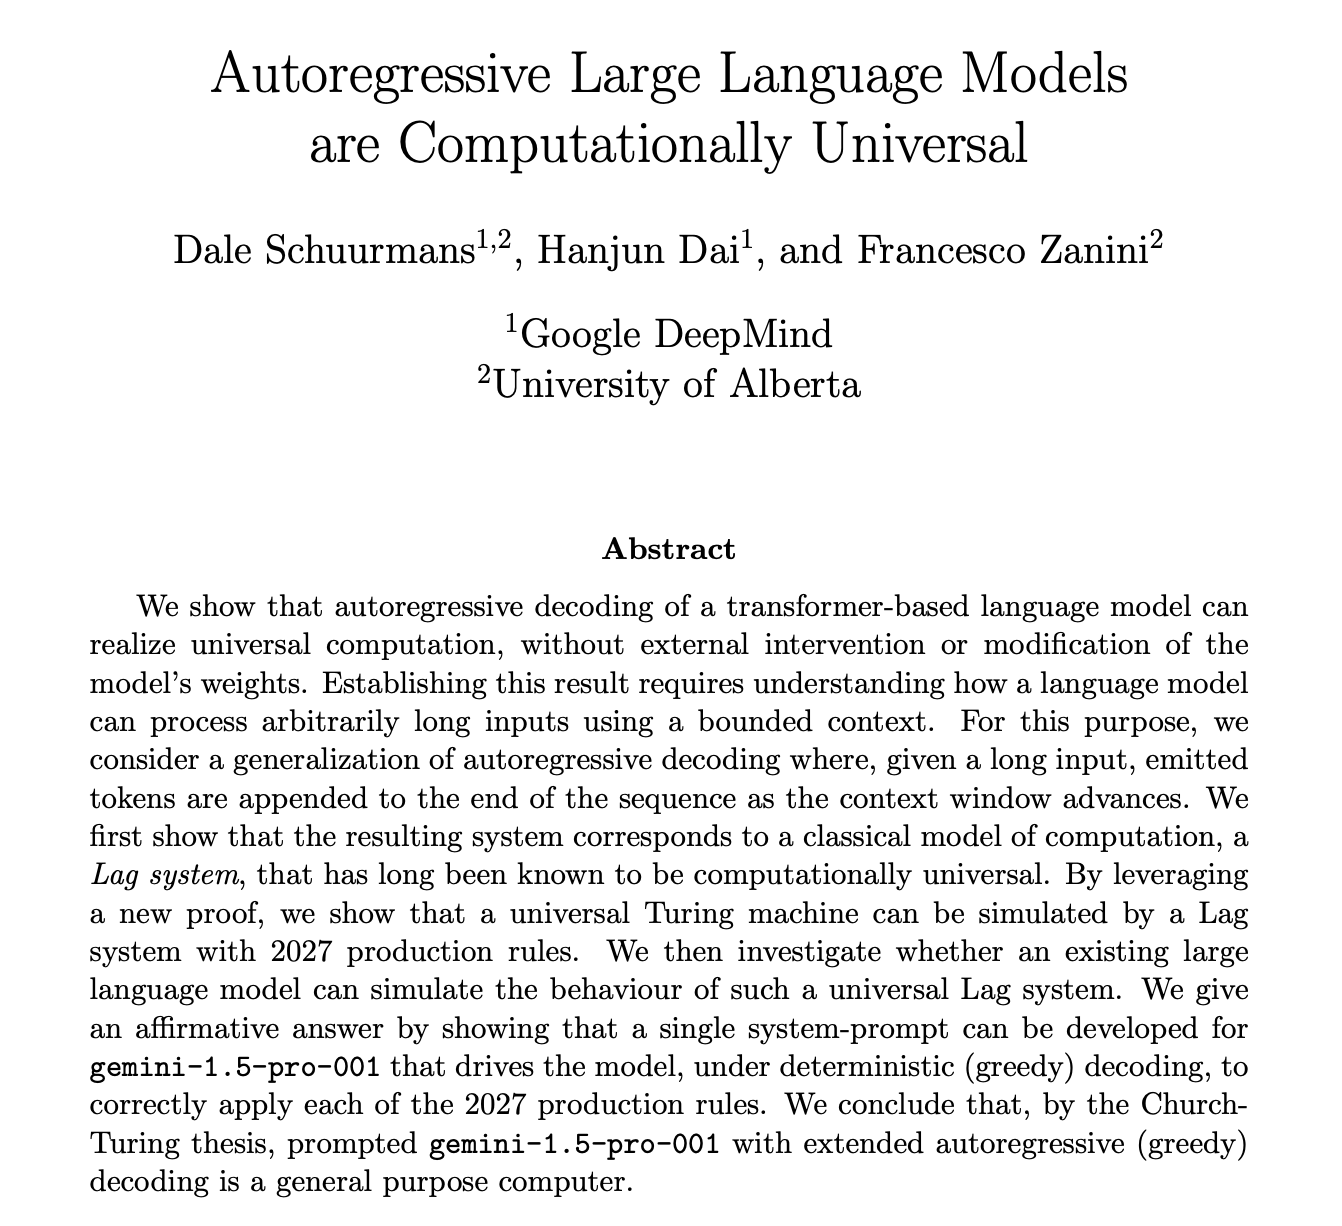
\includegraphics[width=0.62\textwidth]{Figures/AutoLLMs.png}}
    \caption{The paper this lecture is based on \cite{schuurmans2024autoregressive}. Read for more info.}
    \label{fig: 2.1.1}
\end{figure}

\begin{itemize}
    \item Introduction \href{https://youtu.be/ShM-T4oeYjw?si=fsZwObn6LdUuPIMA}{[5:28]}
    \begin{itemize}
        \item Recall Theorem \ref{thm:1.1}, Chain Rule of Probability \href{https://youtu.be/ShM-T4oeYjw?si=xZnM8GOIv6OGB-Ra&t=379}{[6:19]}
        \item The bounded context window defines a K-Markov model \href{https://youtu.be/ShM-T4oeYjw?si=PZ1ZMbLjJaIqu7_Q&t=501}{[8:27]}
        \item Challenge: Figure how to operate a K-Markov model on an input string larger than K
    \end{itemize}
    \item Extend Chain Rule of Prob. to Extended Autoregressive Decoding \href{https://youtu.be/ShM-T4oeYjw?si=e4lvOWzkCGe_ClLH}{[10:10]}
    \begin{itemize}
        \item Idea: Extension generates and append two symbols instead of one
    \end{itemize}
    \item Introduction and Examples of LAG Systems \href{https://youtu.be/ShM-T4oeYjw?si=QOeX4wHOR30GQbBF&t=1271}{[21:11]}
\end{itemize}
\begin{definition}[Lag System]
A Lag system consists of a finite set of rules $x_1...x_N \to y$, where $N$ is the length of the context, $x_1...x_N \in \Sigma^N$ denotes a sequence of symbols to be matched, and $y \in \Sigma^*$ is a corresponding output \cite{schuurmans2024autoregressive}.

For a deterministic Lag system, each pattern $x_1...x_N$ is unique, hence the Lag system defines a partial function $L : \Sigma^N \to \Sigma^*$ that maps a pattern $x_1...x_N$ to a corresponding output y \cite{schuurmans2024autoregressive}.

Lag system computation is defined by operating over a memory string, where in each iteration, a rule is matched to the prefix of the memory string, then the result appended to the string, after which the first symbol is deleted \cite{schuurmans2024autoregressive}.
\end{definition}
\hrule
\textbf{For interesting behavior, we have at least a rule that appends more than 1 symbol.} We also introduce a Halt symbol $H$ to terminate whenever generated. Computation also terminates when there is no rule for the current context, which includes when the current memory string is shorter than $N$.

\begin{itemize}
    \item Lag System Operates Memory as a Queue Machine \href{https://youtu.be/ShM-T4oeYjw?si=kr1ip53SZuYQ0LT0&t=1785}{[29:45]}
    \begin{itemize}
        \item Thus, we can rotate the memory even if the memory is bigger than the context size!
        \item Challenge: The queue machine has no external controller
        \item Challenge: The queue machine can only operate in one direction
        \item \textbf{To simulate a TM, we need to track the current machine state and be able to rotate the memory in both directions!}
    \end{itemize}
    \item Lag System can track the current state and rotate both directions \href{https://youtu.be/ShM-T4oeYjw?si=Htp1M1CRSuv7LrUi&t=2231}{[37:11]}
    \begin{itemize}
        \item Explanation and Simulations \href{https://youtu.be/ShM-T4oeYjw?si=2pF9RDl6k08Ehjk_&t=2575}{[42:55 - 55:10]}
    \end{itemize}
    \item Lag Systems simulates a Turing Machine w/ a cubic time overhead \href{https://youtu.be/ShM-T4oeYjw?si=Ara_vbPniwxN2itp&t=3310}{[55:10]}
    \begin{itemize}
        \item Examples and Simulations \href{https://youtu.be/ShM-T4oeYjw?si=FZf4ewMOwBZ4L3k8&t=3831}{[1:03:51]}
    \end{itemize}
    \item Autoregressive LLM can simulate a Universal LAG System \href{https://youtu.be/ShM-T4oeYjw?si=BXQV-wcwkZz7P8BO&t=4207}{[1:10:07]}
    \begin{itemize}
        \item Brute force: Entire set of rules as a system prompt to LLM \href{https://youtu.be/ShM-T4oeYjw?si=kNkUy45FYvbykU2V&t=4354}{[1:12:34]}
        \item Note: Gemini 1.5 Pro was used due to the large context window.
    \end{itemize}
    \item Questions/Current/Future Work \href{https://youtu.be/ShM-T4oeYjw?si=iPwZ_a8Hqi404gec&t=4538}{[1:15:38]}
    \begin{itemize}
        \item Proof is now done for random LLMs
    \end{itemize}
\end{itemize}

\newpage

\markboth{Appendix A}{Appendix A}
\section*{Appendix A: Extra Proofs and Results}
\addcontentsline{toc}{section}{Appendix A: Extra Proofs and Results}

More appendix content here.

\markboth{Appendix B}{Appendix B}
\section*{Appendix B: Supplementary Figures}
\addcontentsline{toc}{section}{Appendix B: Supplementary Figures}

More appendix content here.

\newpage

\printbibliography
\addcontentsline{toc}{section}{References}

\end{document}
